\documentclass{article}
\usepackage{graphicx} % Required for inserting images
\usepackage{lipsum}
\usepackage{mdframed}
\usepackage{amssymb} % for \checkmark symbol
\usepackage{float}

\usepackage{geometry}
\usepackage{amsmath}
\usepackage{dingbat}
\usepackage{color}
\usepackage{pifont} % for \ding command

\usepackage{array}
\usepackage{booktabs}
\usepackage{enumitem}
\usepackage[colorlinks=true, linkcolor=black, urlcolor=black, citecolor=black]{hyperref}\usepackage{listings}
\lstset{language=verilog}
\usepackage{fancyhdr}
\usepackage{xcolor}
\usepackage{changepage} % Add package to adjust page layout
\geometry{
    top=1in, %sets the top margin to 1 inch
    bottom=1in, %sets the bottom margin to 1 inch
    left=1in, %sets the left margin to 1 inch
    right=1in %sets the right margin to 1 inch
}
\geometry{
    top=0.9in, %sets the top margin to 1 inch
    bottom=0.9in, %sets the bottom margin to 1 inch
    left=1in, %sets the left margin to 1 inch
    right=1in %sets the right margin to 1 inch
}
\lstset{
	language=verilog,
	basicstyle=\ttfamily\small,
	aboveskip={1.0\baselineskip},
	belowskip={1.0\baselineskip},
	columns=fixed,
	extendedchars=true,
	breaklines=true,
	tabsize=4,
	prebreak=\raisebox{0ex}[0ex][0ex]{\ensuremath{\hookleftarrow}},
	frame=lines,
	showtabs=false,
	showspaces=false,
	showstringspaces=false,
	keywordstyle=\color[rgb]{0.627,0.126,0.941},
	commentstyle=\color[rgb]{0.133,0.545,0.133},
	stringstyle=\color[rgb]{01,0,0},
	numbers=left,
	numberstyle=\small,
	stepnumber=1,
	numbersep=10pt,
	captionpos=t,
	escapeinside={\%*}{*)}
}

% Define the colors
\definecolor{codebg}{RGB}{150,200,200}
\definecolor{codeborder}{RGB}{200,200,200}
% Define a new environment for colored code blocks
\newmdenv[%
    backgroundcolor=codebg,%
    linecolor=codeborder,%
    linewidth=2pt,%
    roundcorner=10pt%
]{codeblock}

\pagestyle{fancy}
\fancyhead{} % Clear all header fields
\fancyhead[L]{{\textbf{Deep Learning}}} % Left header
\fancyhead[R]{\text{\textcolor{}{\textbf{Final project} }}} % Right header
\setlength{\headheight}{20pt} % Set header height.
\fancyfoot[C]{}

\fancyfoot[L]{\textit{\small Brown CSCI 1470: Deep Learning}}
\fancyfoot[R]{\thepage}
\renewcommand{\footrulewidth}{0.4pt} % Width of the line
\begin{document}
\begin{figure}
    \centering
    
\includegraphics[width=0.8\textwidth]{brown_graduate_school_logo.pdf}
    \label{fig:brown_graduate_school_logo}
\end{figure}

\title{\huge\bf CSCI 1470 \\ \color{teal} Deep Learning - SPRING 2025\\
\color{red} 
Final Project:
\color{}\normalize Learning to Play Pinball with MuZero\\}
\author{\Large\bf Guanghe (Eric) Fan | Hatem Mohamed | Shivam Hingorani}
\date{April/May 2025}
\maketitle{}
\newpage
\tableofcontents
\newpage
%%%%%%%%%%%%%%%%%%%%%%%%%%%%%%%%%%%%%%%%%%%%%%%%%%%%%%%%%%%%%%%%%%%%%%%%%%%%%5
\section{Introduction}
Our goal for this project was to build a reinforcement learning agent capable of playing digital pinball autonomously. Pinball presents a challenging environment that requires fine motor control and long-term strategic planning in the face of chaotic physics. We approached this using the MuZero algorithm, a state-of-the-art model-based RL technique from Google DeepMind. Unlike traditional methods, MuZero learns to predict optimal value, reward, and policy from observations without needing the environment's rules. We chose MuZero for its performance in complex tasks such as Atari, Go, and Chess, and its potential for real-time physics-driven games such as pinball.

\subsection{Pinball}
Pinball is a fast-paced arcade game in which players use flippers to control a ball on a sloping field, scoring points by hitting targets while avoiding the drain. Success requires timing, accuracy, and an understanding of the ball's interactions within the game environment. Despite its apparent simplicity, Pinball is a sophisticated, skill-based game that combines strategy, physics, and quick reflexes. A sample environment from this game is shown below.

\begin{figure}[H]
    \centering
    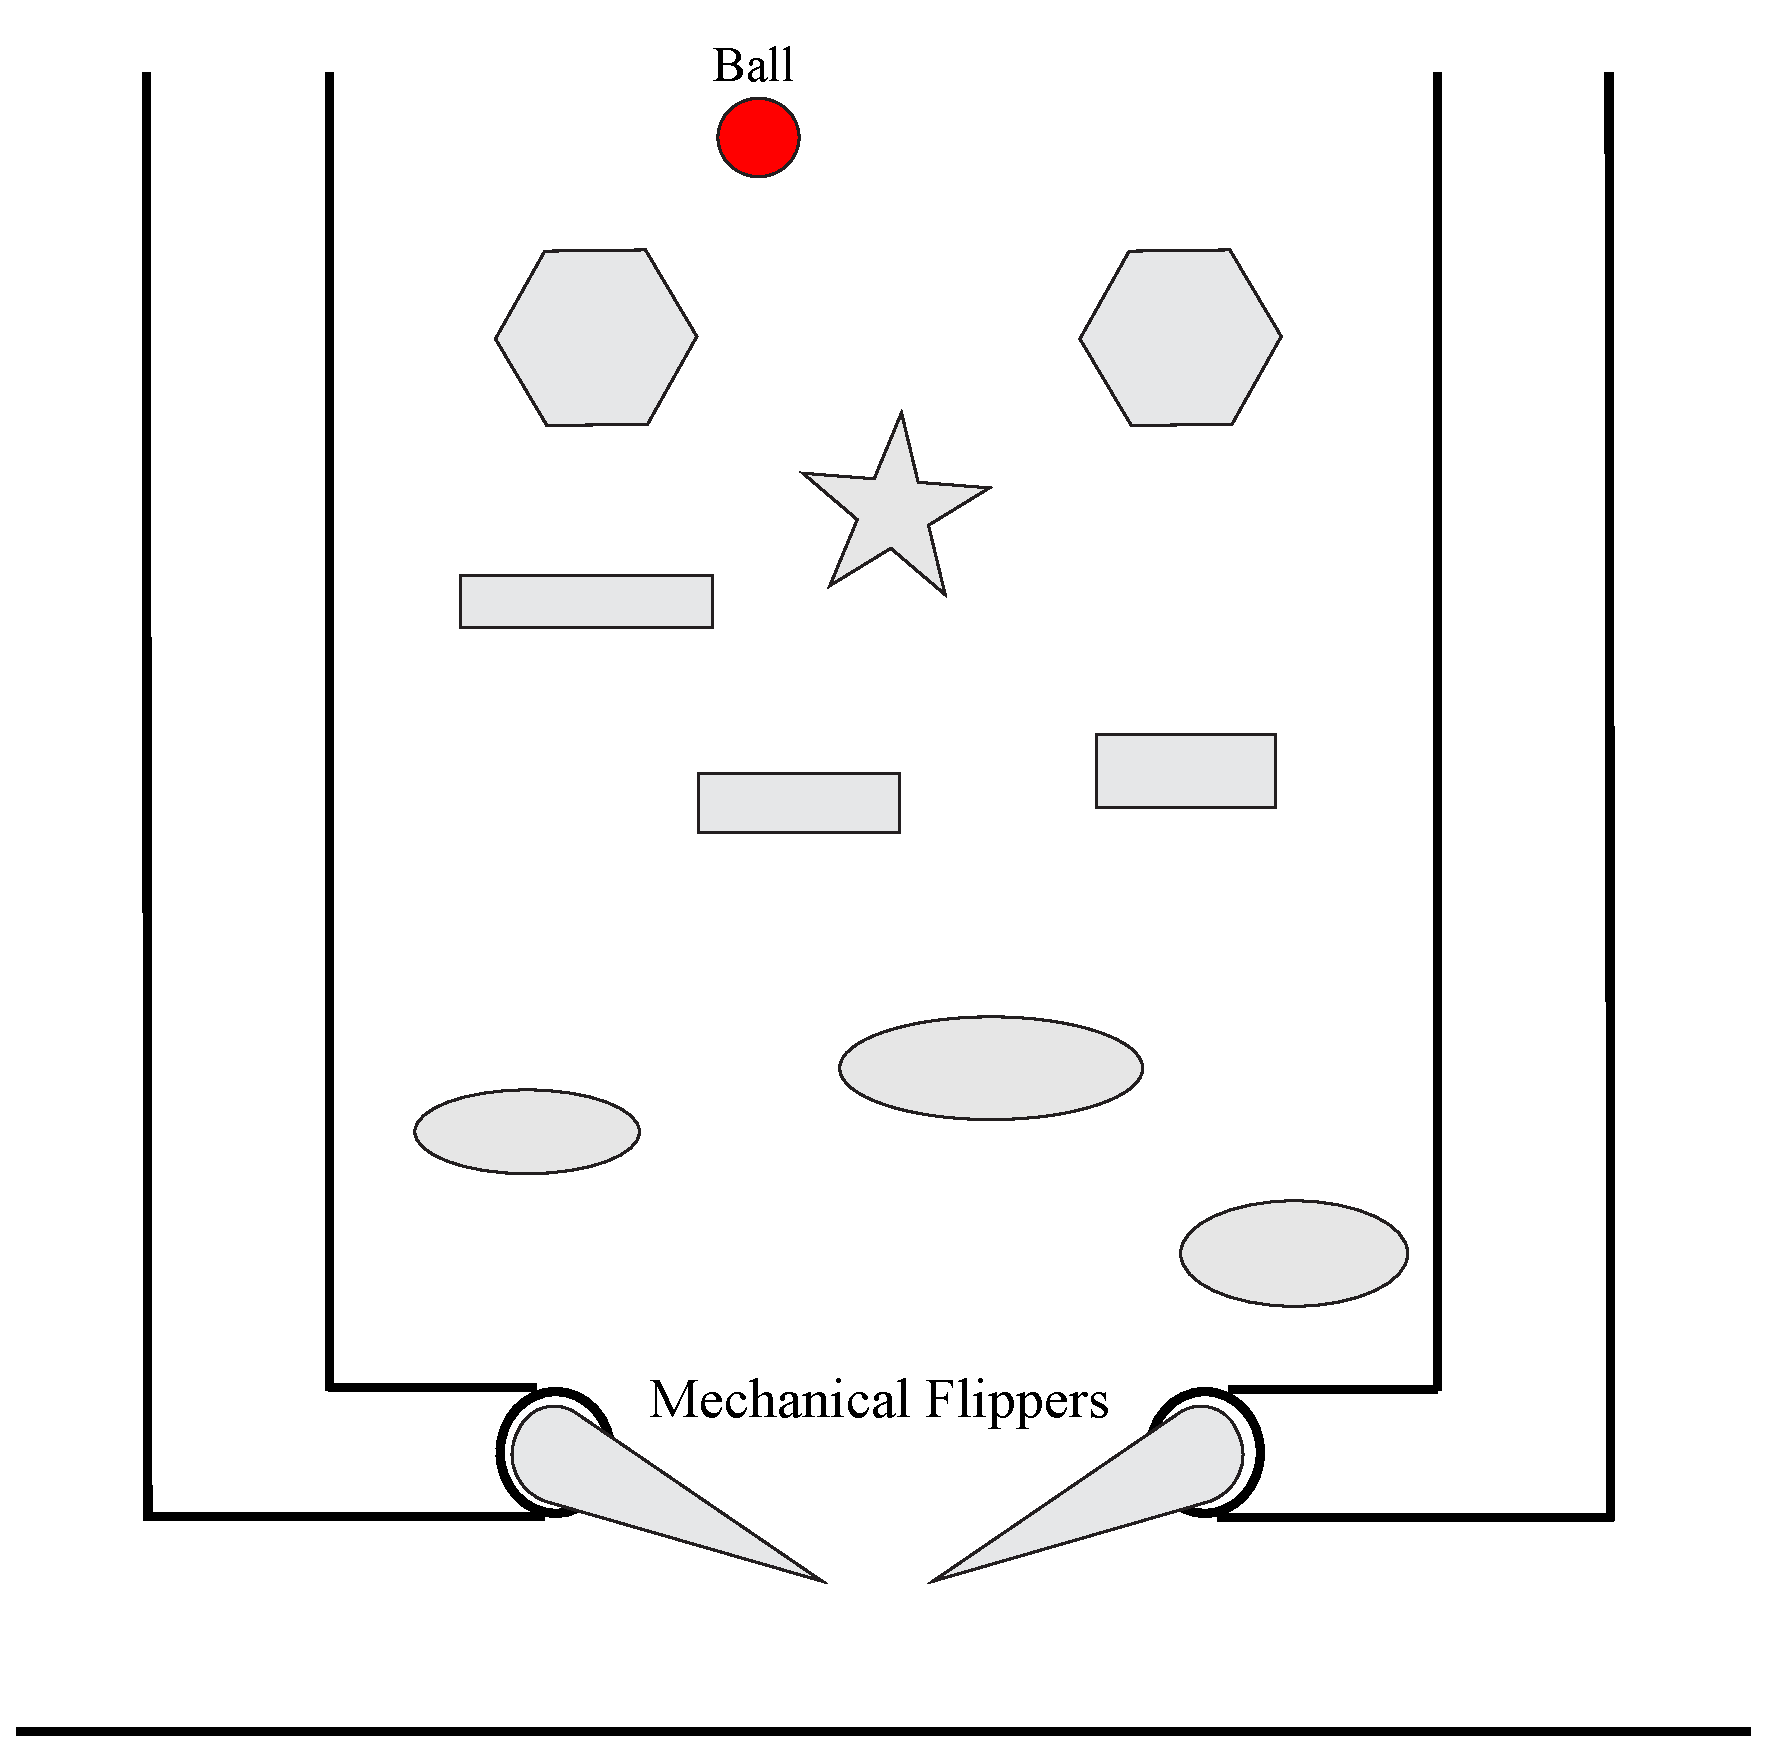
\includegraphics[width=0.9\textwidth]{pinball_example.pdf}
    \caption{Pinball involves a ball interacting with a variety of obstacles, targets, and other environmental factors, such as gravity.}
    \label{fig:pinball_example}
\end{figure}

\subsection{Reinforcement Learning and MuZero}
Reinforcement Learning (RL) is a branch of machine learning wherein an agent learns to maximize the cumulative reward through trial and error. The merits of RL have often been demonstrated in the context of gaming:
\begin{itemize}
    \item AlphaGo used RL to defeat human champions in the game of Go.
    \item Deep Q-Networks (DQN) learned to play Atari 2600 games directly from raw pixels and score data.
    \item MuZero, a more advanced algorithm, mastered games such as Chess, Shogi, and several Atari titles without knowing the rules in advance.
\end{itemize}
These successes, among many others, demonstrate RL's ability to handle complex, high-dimensional environments that need strategy and planning.

MuZero is especially interesting for its ability to learn to navigate environments without given rules. Rather than requiring a model of environment dynamics beforehand, it uses self-play to build a condensed internal model relevant for decision making. It then predicts future rewards, values, and policies by combining representation learning with planning. MuZero has shown remarkable performance in both discrete and continuous action spaces.

MuZero relies on the Monte Carlo Tree Search (MCTS) to predict and assess future action sequences based on its learning. MCTS extends a search tree from the current latent state, using the prediction network for value and policy estimates and the dynamics network to simulate future states. It uses the Upper Confidence Bound (UCB) formula to balance exploration and exploitation. By choosing the action with the highest visit count from the root level, MuZero combines planning and learning for informed judgments.

\section{Methodology}
Our project is based on the MuZero architecture, which seamlessly integrates learning and planning through three interconnected Convolutional Neural Networks (CNNs): the representation network, the dynamics network, and the prediction network. The representation network processes raw observations, such as game frames, and encodes them into a compact latent state using convolutional layers. The dynamics network takes this latent state along with an action to predict the subsequent latent state and the immediate reward, thereby modeling the internal transitions of the environment. The prediction network operates on the latent state to output a probability distribution over possible actions (policy head) and an estimated expected return (value head). These three networks are trained jointly using samples drawn from a replay buffer.

MuZero performs unrolling by recursively applying the dynamics and prediction networks for a predetermined number of future steps (typically five in our implementation) to simulate and learn from hypothetical sequences of actions. The training loss is calculated based on the predicted values, rewards, and policies at each step of the unroll and is then backpropagated. For making decisions within the environment, MuZero utilizes MCTS to simulate potential future paths of action. The action that is visited most frequently from the root of the MCTS tree is chosen and executed. This combined approach allows the agent to learn how to play pinball effectively without any prior knowledge of the game's physics.

\begin{figure}[H]
    \centering
    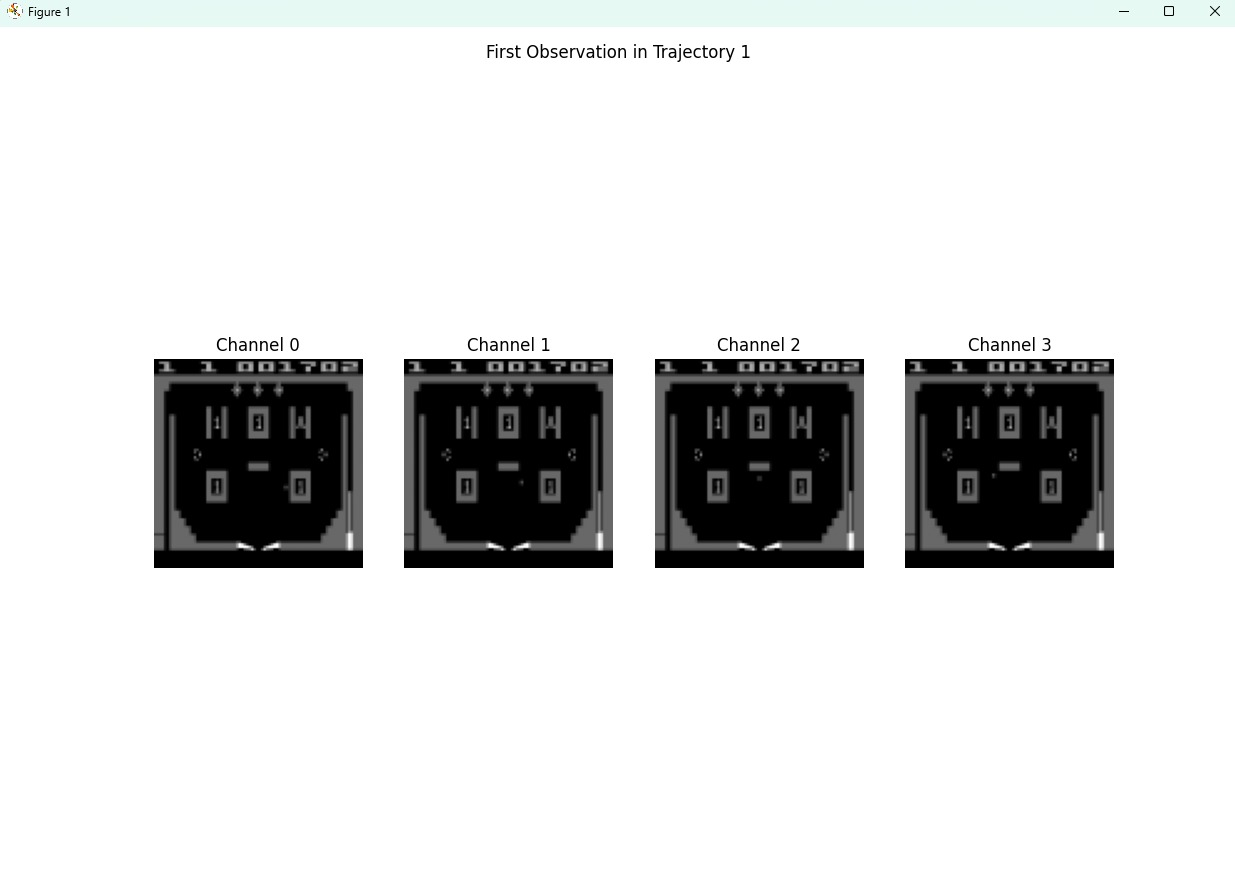
\includegraphics[width=1.0\textwidth]{pinball_training.jpeg}
    \caption{MuZero trains by capturing the game state at every timestep of self-play.}
    \label{fig:pinball_training}
\end{figure}

\subsection{Optimizations}
MuZero's architecture utilizes deep convolutional residual networks (ResNets) for its constituent parts. The representation network encodes observations using convolutional layers augmented with residual connections. The dynamics network employs similar ResNet blocks to predict the next latent state and the reward. The prediction network, also based on ResNets, outputs the policy and value estimates. These structural elements are crucial for modeling complex dynamics and facilitating planning through internal simulations, all without requiring explicit rules of the environment.

However, the computational demands of the original MuZero algorithm, stemming from the large search tree and deep residual blocks, necessitated significant optimizations to conform to the scope of this project and our resources. These simplifications included replacing some residual blocks with standard convolutional networks to simplify the model, resulting in a smaller CNN that could be trained on less demanding hardware like a laptop or a single GPU. Furthermore, our implementation performs only 50 MCTS simulations per move, a substantial reduction compared to the original MuZero's 800, which significantly reduces inference time. While further reduction is possible, it would likely impact the accuracy of the agent's planning.

\subsection{Technical Specifications}
\begin{itemize}
    \item \textbf{Dataset/Environment:} The game used for training and evaluation was Video Pinball, accessed via the PyGame Learning Environment.
    \item \textbf{Preprocessing:} Involved converting frames to grayscale, resizing them to 84x84 pixels, and stacking four consecutive frames to capture temporal information.
    \item \textbf{Model Architecture:}
    \begin{itemize}
        \item \underline{Representation Network:} A CNN designed to encode the raw observation into a compressed hidden state.
        \item \underline{Dynamics Network:} Predicts the transition to the next hidden state and the reward received after taking an action.
        \item \underline{Prediction Network:} Outputs the probability distribution over possible actions (policy) and an estimated value of the current state.
    \end{itemize}
    \item \textbf{Training Pipeline:} Consists of several key stages: Self-Play to generate game trajectories, a Replay Buffer to store collected experiences, and Training, which involves sampling mini-batches from the buffer and computing losses for reward, value, and policy predictions.
\end{itemize}

\begin{figure}[H]
    \centering
    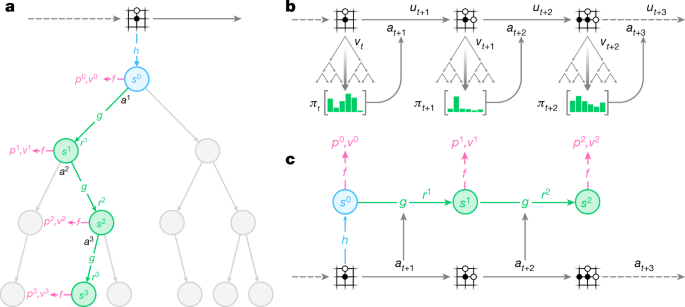
\includegraphics[width=0.8\textwidth]{muzero.png}
    \caption{The MuZero model architecture.}
    \label{fig:muzuro}
\end{figure}

\section{Challenges}
The most significant challenge we faced throughout the project was managing the substantial time and computational resources required for training a MuZero agent, particularly in a complex environment like pinball. Training even our simplified version of MuZero proved to be far more computationally intensive than we expected, resulting in lengthy training cycles that slowed down the process of iteration and debugging. Integrating the Monte Carlo Tree Search (MCTS) component was also a notable difficulty. To mitigate the long training times, we adopted a strategy of validating our implementation on a simpler game, Breakout, taking advantage of the modular architecture and the abstraction afforded to us by the PyGame Learning Environment. This approach enabled us to confirm that the core pipeline was functioning correctly before deploying it on the more computationally demanding Pinball environment.

\begin{figure}[H]
    \centering
    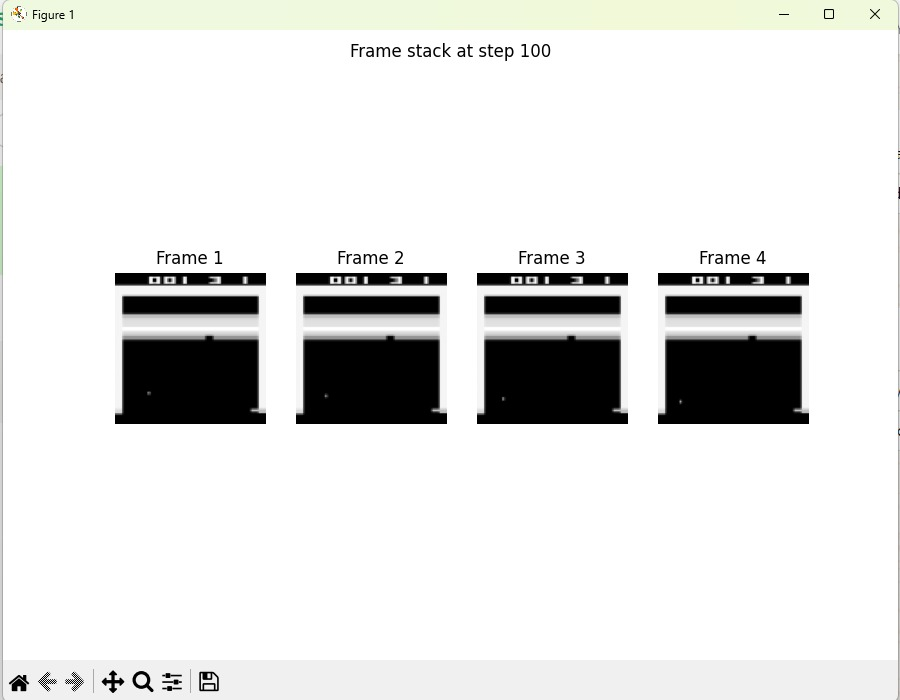
\includegraphics[width=0.8\textwidth]{breakout_training.jpeg}
    \caption{To accelerate our training progress, we first trained our agent to play Breakout.}
    \label{fig:breakout_training}
\end{figure}
\begin{figure}[H]
    \centering
    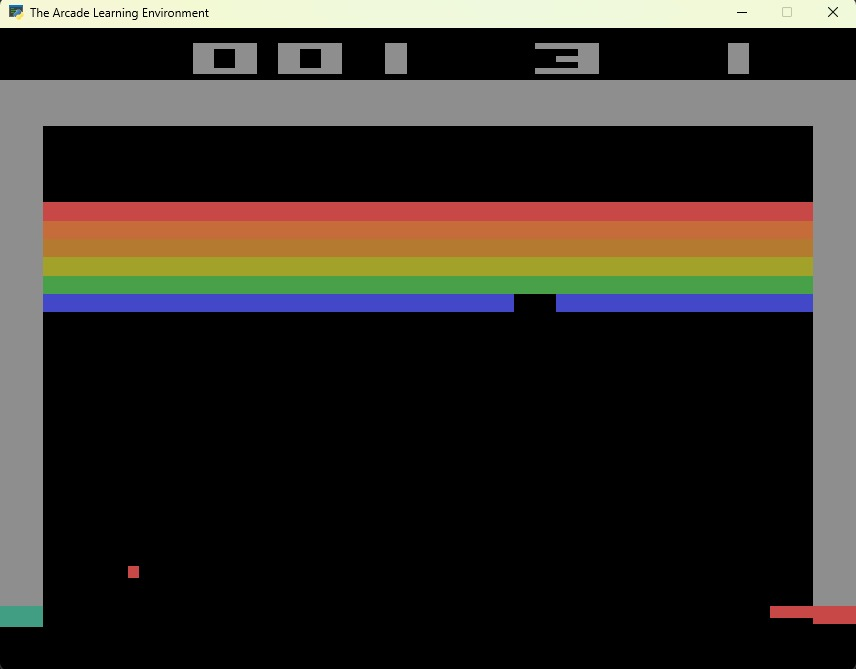
\includegraphics[width=0.8\textwidth]{breakout_gameplay.jpeg}
    \caption{Our agent plays Breakout sufficiently well for autonomous deployment.}
    \label{fig:breakout_gameplay}
\end{figure}

Having built confidence in our network, we then attempted to deploy a longer-term training job on the Oscar computing cluster. However, even with the increased computing power, it quickly became clear that pinball's exponentially greater complexity would require us to go beyond the timeline of this project. While we were able to confirm that our model runs as expected and can make progress toward learning a game as complex as pinball, we simply did not have the time that was necessary to train the model to achieve results as strong as those of our training on Breakout.

\section{Results}
In looking at the more complete results of training our model on Breakout, we found that the training loss, while initially high, showed a significant decrease after approximately ten epochs. Notable fluctuations continue to occur through the end of our training job, and b the 60th epoch, the training loss generally stabilizes below 1.0 in most cases, indicating that the model is effectively learning from the potentially noisy data generated during self-play. In evaluating the model's performance more qualitatively, we found that the model could last thousands of timesteps, successfully rivaling the performance of a human.

These results indicated that the core components, specifically the replay buffer and trainer modules, are operational, and the training process runs successfully. The drastic oscillations in the loss curve are anticipated given the nature of reinforcement learning training. There remains potential for improving our MCTS implementation (more on this later), but the underlying infrastructure is robust and prepared for more complex training jobs.

\begin{figure}[H]
    \centering
    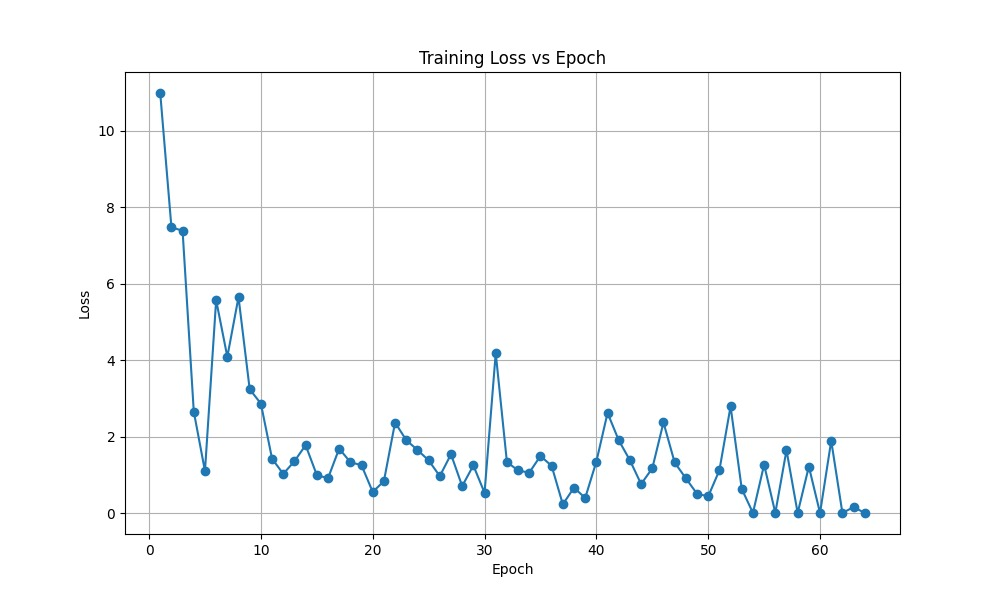
\includegraphics[width=1.0\textwidth]{loss_graph.jpeg}
    \caption{After some initial fluctuations, our training process stabilizes – a promising result.}
    \label{fig:loss_graph}
\end{figure}

When transitioning to pinball, early results are expectedly weak, with losses in the realm of 1500. Over the few hours spent training our network to play pinball, we noticed a significant improvement in our loss measure, but the model was still far from ready for autonomous deployment. We remain confident, however, that given sufficient time and compute resources, our model would learn to play pinball as well as a human competitor.

\begin{figure}[H]
    \centering
    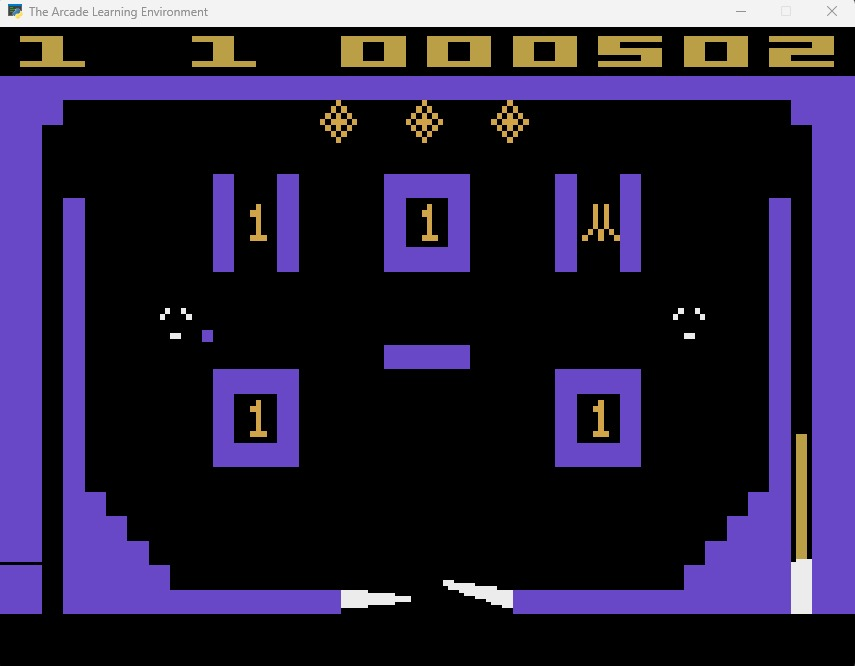
\includegraphics[width=0.9\textwidth]{pinball_gameplay.jpeg}
    \caption{Per our expectations, the model successfully trains and plays pinball, though with weak performance). Given more time and computing resources, this model would eventually learn to play pinball as well as we trained it to play Breakout.}
    \label{fig:pinball_gameplay}
\end{figure}

\section{Reflection}
Overall, we feel that our project successfully resulted in the implementation of a simplified MuZero pipeline, effectively adapted to the new domain of digital pinball. In relation to our defined goals, we successfully achieved the base goal: the agent learned non-random behavior and demonstrated the ability to achieve consistent reward. While the agent is not yet playing at a competitive level (which was our target goal), the foundational infrastructure is in place, providing a solid basis for future training and optimization efforts that could potentially lead to reaching or even exceeding this goal. The stretch goal of achieving generalization across different pinball layouts was not explicitly addressed within the scope of this project but remains a promising direction for future work.

Regarding whether the model worked out as expected, the initial behavior of the agent without the integrated MCTS planning was qualitatively not as strong as we might have hoped, as it did not immediately demonstrate skilled gameplay. However, the quantitative results, particularly the decreasing training loss, clearly indicate that the core learning components are functioning correctly and that the model is indeed learning effectively from the training data.

Our approach evolved over the course of the project, primarily through the strategic decision to validate the core architecture and training pipeline on a simpler game, Breakout. This pivot was essential for managing the computational cost and accelerating the iteration and debugging cycle before committing to the longer training times required for the more complex Pinball environment. If we were to undertake this project again, we might consider integrating the MCTS component earlier in the development process, perhaps initially testing it within the simpler environment, to gain earlier insights into the impact of planning on the agent's performance.

If we had additional time to continue working on this project, our primary focus would be on refining the Monte Carlo Tree Search (MCTS) implementation. This would involve incorporating techniques such as Dirichlet exploration noise and tuning the temperature parameter for softmax sampling to improve exploration and policy learning. Further fine-tuning of the rollout steps within MCTS and the overall learning rate of the training process would also be beneficial areas for optimization. Developing deeper network architectures for the representation, dynamics, and prediction networks is another avenue for potential improvement. Finally, a key future direction would be to evaluate and potentially enhance the agent's ability to generalize its learned strategy to different pinball table layouts.

Our biggest takeaways from this project include a deeper understanding of the complexities involved in implementing state-of-the-art reinforcement learning algorithms like MuZero. We learned firsthand the critical importance of effectively managing computational resources when working with such models and the significant value of adopting a modular design approach and validating components on simpler environments before scaling up. Overall, we gained valuable practical experience in the challenges and intricacies of training deep reinforcement learning agents to tackle complex, dynamic tasks.

\end{document}